\newif\ifglobal

%%%%%%%%%%%%%%%%%%%%%%%
%%% Compile to view %%%
%%%%%%%%%%%%%%%%%%%%%%%

%%%%%%%%%%%%%%%%%%%%%%%%%%%%%%%%%%%%%%%%%%%%%%%%%%%
%%% Readme:                                     %%%
%%% https://www.overleaf.com/read/bwdjvfjksvjy/ %%%
%%%%%%%%%%%%%%%%%%%%%%%%%%%%%%%%%%%%%%%%%%%%%%%%%%%

% >>> M?: marks a module setting number or important notice

% >>> M4: Set {./relative-path} to external files for this module <<<
\def \modulefiles {./01-ULP}
% To add an external file, use:
% (Replace '---' with actual filename)
% '\input{\modulefiles/tables/---.tex}' for tables
% '\includegraphics{\modulefiles/figures/---}' for figures
% '\subfile{\modulefiles/---}' for register files

% >>> M1: This module is in global project? <<<
% 'YES' - uncomment; 'NO' - comment out
\globaltrue

\ifglobal
    \documentclass[main\_\_EN.tex]{subfiles}

\else
    \documentclass[openany, 10pt]{book}

    % >>> M2: In ./00-shared/preamble-trm-module, also find
    %         settings for visibility of todo notes, watermark <<<
    \usepackage{preamble-trm-module}

    % >>> M3: Temporary labels in English,
    %         you can add your own labels there <<<
    \myexternaldocument{./00-shared/temp-labels-en}

\fi %\ifglobal


\setcounter{secnumdepth}{4}


% Define formatting of parts and chapters in text
\setenglishformatting


% >>> M5: If this module needs any updates in
% './00-shared/preamble-trm-module.sty'
% (include additional package, etc.), contact your module PM
% or create the file './00-shared/changelog.tex' make the
% necessary updates yourself and document them in this file <<<

% Make text left-aligned and allow latex to break pages naturally, comment out for full justification
\raggedright
\raggedbottom


\begin{document}


% Sets language into which pre-defined bits of text are translated
\selectlanguage{english}

% Do not delete this block
\ifglobal
% Add the following front matter if
% this module is outside of global project
\else
    \InputIfFileExists{readme}{}{}
    \listoftodos
    {\let\clearpage\relax \listofdonetodos}
    \tableofcontents
    %\listoftables
    %\listoffigures
\fi


%%%%%%%%%%%%%%%%%%%%%%%%%
%%% TRM Module Begins %%%
%%%%%%%%%%%%%%%%%%%%%%%%%

\hypertarget{ulp}{}
\chapter{ULP Coprocessor (ULP)}
\label{mod:ulp}

\section{Introduction}

The ULP coprocessor is an ultra-low-power processor that remains powered on during the Deep-sleep mode of the main SoC. Hence, the developer can store in the RTC memory a program for the ULP coprocessor to access peripheral devices, internal sensors and RTC registers during deep sleep. This is useful for designing applications where the CPU needs to be woken up by an external event, or timer, or a combination of these, while maintaining minimal power consumption.

\section{Features}

\begin{itemize}
    \item Contains up to 8 KB of SRAM for instructions and data
    \item Uses RTC\_FAST\_CLK, which is 8 MHz
    \item Works both in normal and deep sleep
    \item Is able to wake up the digital core or send an interrupt to the CPU
    \item Can access peripheral devices, internal sensors and RTC registers
    \item Contains four 16-bit general-purpose registers (R0, R1, R2, R3) for manipulating data and accessing memory
    \item Includes one 8-bit Stage\_cnt register which can be manipulated by ALU and used in JUMP instructions
\end{itemize}

\begin{figure}[H]
    \centering
    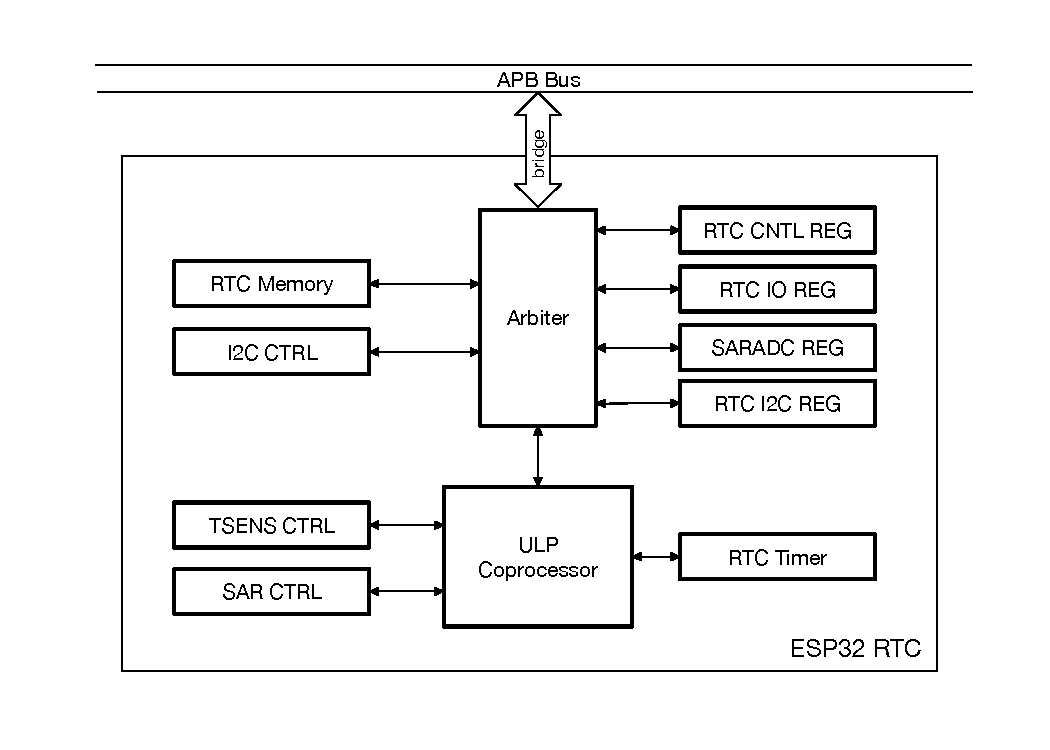
\includegraphics[width=0.8\textwidth]{./01-ULP/figures/ulp_cp.pdf}
    \caption{ULP Coprocessor Diagram}
    \label{figure:ULP coprocessor}
\end{figure}


\section{Functional Description}

The ULP coprocessor is a programmable FSM (Finite State Machine) that can work during deep sleep. Like general-purpose CPUs, ULP coprocessor also has some instructions which can be useful for a relatively complex logic, and also some special commands for RTC controllers/peripherals. The 8 KB of SRAM RTC slow memory can be accessed by both the ULP coprocessor and the CPU; hence, it is usually used to store instructions and share data between the ULP coprocessor and the CPU.

The ULP coprocessor can be started by software or a periodically-triggered timer. The operation of the ULP coprocessor is ended by executing the \hyperref[subsection:HALT]{HALT} instruction. Meanwhile, it can access almost every module in RTC domain, either through built-in instructions or RTC registers. In many cases the ULP coprocessor can be a good supplement to, or replacement of, the CPU, especially for power-sensitive applications. Figure \ref{figure:ULP coprocessor} shows the overall layout of a ULP coprocessor.


\section{Instruction Set}

The ULP coprocessor provides the following instructions:

\begin{itemize}
    \item Perform arithmetic and logic operations - ALU
    \item Load and store data - LD, ST, REG\_RD and REG\_WR
    \item Jump to a certain address - JUMP
    \item Manage program execution - WAIT/HALT
    \item Control sleep period of ULP coprocessor  - SLEEP
    \item Wake up/communicate with SoC - WAKE
    \item Take measurements - ADC
    \item Communicate using I2C - I2C\_RD/I2C\_WR
\end{itemize}

The ULP coprocessor's instruction format is shown in Figure \ref{figure:ULP-instruction}.

\begin{figure}[H]
    \centering
    \begin{bytefield}{32}
        \bitheader[bitformatting={\scriptsize}]{0,27,28,31} \\
        \bitbox{4}{\it{OpCode}} & \bitbox{28}{\it{Operands}}
    \end{bytefield}
    \caption{The ULP Coprocessor Instruction Format}
    \label{figure:ULP-instruction}
\end{figure}

 An instruction, which has one \textit{OpCode}, can perform various different operations, depending on the setting of \textit{Operands} bits. A good example is the \hyperref[subsection:ALU]{ALU} instruction, which is able to perform 10 arithmetic and logic operations; or the \hyperref[subsection:JUMP]{JUMP} instruction, which may be conditional or unconditional, absolute or relative.

Each instruction has a fixed width of 32 bits. A series of instructions can make a program be executed by the ULP coprocessor. The execution flow inside the program uses 32-bit addressing. The program is stored in a dedicated region called Slow Memory (RTC\_SLOW\_MEM), which is visible to the main CPUs as one that has an address range of 0x5000\_0000 to 0x5000\_1FFF (8 KB).

The \textit{OpCode} in this chapter is represented by 4'd\textcolor{red}{\textit{x}}, where 4 stands for 4-bit width, 'd is a decimal symbol, \textcolor{red}{\textit{x}} stands for the value of \textit{OpCode} (\textcolor{red}{\textit{x}}: 0 \verb+~+ 15).

\subsection{ALU - Perform Arithmetic/Logic Operations} \label{subsection:ALU}

The ALU (Arithmetic and Logic Unit) performs arithmetic and logic operations on values stored in ULP coprocessor registers, and on immediate values stored in the instruction itself. \\
The following operations are supported:
\begin{itemize}
    \item Arithmetic: ADD and SUB
    \item Logic: bitwise logical AND and bitwise logical OR
    \item Bit shifting: LSH and RSH
    \item Moving data to register: MOVE
    \item Stage count register manipulation: STAGE\_RST, STAGE\_INC and STAGE\_DEC
\end{itemize}

The ALU instruction, which has one \textit{OpCode}, can perform various different arithmetic and logic operations, depending on the setting of the instruction's bits [27:21] accordingly.


\subsubsection{Operations Among Registers}

\begin{figure}[H]
    \centering
    \begin{bytefield}{32}
        \bitheader[bitformatting={\scriptsize}]{0,1,2,3,4,5,21,24,25,27,28,31} \\
        \bitbox{4}{4'd7} & \bitbox{3}{3'b0} & \bitbox{4}{ALU\_sel} & \bitbox{15}{} & \bitbox{2}{Rsrc2} & \bitbox{2}{Rsrc1} & \bitbox{2}{Rdst}
    \end{bytefield}
    \caption{Instruction Type — ALU for Operations Among Registers}
    \label{figure:ALU-among-registers}
\end{figure}

When bits [27:25] of the instruction in Figure \ref{figure:ALU-among-registers} are set to 3'b0, ALU performs operations, using the ULP coprocessor register R[0-3]. The types of operations depend on the setting of the instruction's bits [24:21] presented in Table \ref{table:ALU-among-registers}.

\begin{tabular}{ l l }
\textbf{Operand} & \textbf{Description} - see Figure \ref{figure:ALU-among-registers} \\
\textit{ALU\_sel} & Type of ALU operation \\
\textit{Rdst} & Register R[0-3], destination \\
\textit{Rsrc1} & Register R[0-3], source \\
\textit{Rsrc2} & Register R[0-3], source
\end{tabular}

\begin{table}[H]
    \centering
    \begin{tabular}{ c l l l }
    \textbf{ALU\_sel} & \textbf{Instruction} & \textbf{Operation} & \textbf{Description} \\ \hline
    0 & ADD & \textit{Rdst} = \textit{Rsrc1} + \textit{Rsrc2} & Add to register \\
    1 & SUB & \textit{Rdst} = \textit{Rsrc1} - \textit{Rsrc2} & Subtract from register \\
    2 & AND & \textit{Rdst} = \textit{Rsrc1} \& \textit{Rsrc2} & Bitwise logical AND of two operands \\
    3 & OR & \textit{Rdst} = \textit{Rsrc1} | \textit{Rsrc2} & Bitwise logical OR of two operands \\
    4 & MOVE & \textit{Rdst} = \textit{Rsrc1} & Move to register \\
    5 & LSH & \textit{Rdst} = \textit{Rsrc1} \textless\textless\  \textit{Rsrc2} & Bit shifting Left \\
    6 & RSH & \textit{Rdst} = \textit{Rsrc1} \textgreater\textgreater\  \textit{Rsrc2} & Bit shifting Right \\
    \end{tabular}
    \caption{ALU Operations Among Registers}
    \label{table:ALU-among-registers}
\end{table}

\textbf{Note:}
\begin{itemize}
    \item ADD/SUB operations can be used to set/clear the overflow flag in ALU.
    \item All ALU operations can be used to set/clear the zero flag in ALU.
\end{itemize}


\subsubsection{Operations with Immediate Value}

\begin{figure}[H]
    \centering
    \begin{bytefield}{32}
        \bitheader[bitformatting={\scriptsize}]{0,1,2,3,4,19,21,24,25,27,28,31} \\
        \bitbox{4}{4'd7} & \bitbox{3}{3'b1} & \bitbox{4}{ALU\_sel} & \bitbox{1}{} & \bitbox{16}{Imm} & \bitbox{2}{Rsrc1} & \bitbox{2}{Rdst}
    \end{bytefield}
    \caption{Instruction Type — ALU for Operations with Immediate Value}
    \label{figure:ALU-with-immediate-value}
\end{figure}

When bits [27:25] of the instruction in Figure \ref{figure:ALU-with-immediate-value} are set to 3'b1, ALU performs operations, using register R[0-3] and the immediate value stored in [19:4]. The types of operations depend on the setting of the instruction's bits [24:21] presented in Table \ref{table:ALU-with-immediate-value}.

\begin{tabular}{ l l }
\textbf{Operand} & \textbf{Description} - see Figure \ref{figure:ALU-with-immediate-value} \\
\textit{ALU\_sel} & Type of ALU operation \\
\textit{Rdst} & Register R[0-3], destination \\
\textit{Rsrc1} & Register R[0-3], source \\
\textit{Imm} & 16-bit signed value
\end{tabular}

\begin{table}[H]
    \centering
    \begin{tabular}{ c l l l }
    \textbf{ALU\_sel} & \textbf{Instruction} & \textbf{Operation} & \textbf{Description} \\ \hline
    0 & ADD & \textit{Rdst} = \textit{Rsrc1} + \textit{Imm} & Add to register \\
    1 & SUB & \textit{Rdst} = \textit{Rsrc1} - \textit{Imm} & Subtract from register \\
    2 & AND & \textit{Rdst} = \textit{Rsrc1} \& \textit{Imm} & Bitwise logical AND of two operands \\
    3 & OR & \textit{Rdst} = \textit{Rsrc1} | \textit{Imm} & Bitwise logical OR of two operands \\
    4 & MOVE & \textit{Rdst} = \textit{Imm} & Move to register \\
    5 & LSH & \textit{Rdst} = \textit{Rsrc1} \textless\textless\  \textit{Imm} & Bit shifting left \\
    6 & RSH & \textit{Rdst} = \textit{Rsrc1} \textgreater\textgreater\  \textit{Imm} & Bit shifting right \\
    \end{tabular}
    \caption{ALU Operations with Immediate Value}
    \label{table:ALU-with-immediate-value}
\end{table}

\textbf{Note:}
\begin{itemize}
    \item ADD/SUB operations can be used to set/clear the overflow flag in ALU.
    \item All ALU operations can be used to set/clear the zero flag in ALU.
\end{itemize}


\subsubsection{Operations with Stage Count Register} \label{ALU-stage-count}

\begin{figure}[H]
    \centering
    \begin{bytefield}{32}
        \bitheader[bitformatting={\scriptsize}]{4,11,21,24,25,27,28,31} \\
        \bitbox{4}{4'd7} & \bitbox{3}{3'b2} & \bitbox{4}{ALU\_sel} & \bitbox{9}{} & \bitbox{8}{Imm} & \bitbox{4}{}
    \end{bytefield}
    \caption{Instruction Type — ALU for Operations with Stage Count Register}
    \label{figure:ALU-with-stage-count}
\end{figure}

ALU is also able to increment/decrement by a given value, or reset the 8-bit register Stage\_cnt. To do so, bits [27:25] of instruction in Figure \ref{figure:ALU-with-stage-count} should be set to 3'b2. The type of operation depends on the setting of the instruction's bits [24:21] presented in Table \ref{table:ALU-with-stage-count}. The Stage\_cnt is a separate register and is not a part of the instruction in Figure \ref{figure:ALU-with-stage-count}.

\begin{tabular}{ l l }
\textbf{Operand} & \textbf{Description} - see Figure \ref{figure:ALU-with-stage-count} \\
\textit{ALU\_sel} & Type of ALU operation \\
\textit{Stage\_cnt} & Stage count register, a separate register [7:0] used to store variables, such as loop index\\
\textit{Imm} & 8-bit value
\end{tabular}

\begin{table}[H]
    \centering
    \begin{tabular}{ c l l l }
    \textbf{ALU\_sel} & \textbf{Instruction} & \textbf{Operation} & \textbf{Description} \\ \hline
    0 & STAGE\_INC & \textit{Stage\_cnt} = \textit{Stage\_cnt} + \textit{Imm} & Increment stage count register \\
    1 & STAGE\_DEC & \textit{Stage\_cnt} = \textit{Stage\_cnt} - \textit{Imm} & Decrement stage count register \\
    2 & STAGE\_RST & \textit{Stage\_cnt} = 0 & Reset stage count register
    \end{tabular}
    \caption{ALU Operations with Stage Count Register}
    \label{table:ALU-with-stage-count}
\end{table}
\vspace{2em}

\subsection{ST – Store Data in Memory}\label{st instruction}

\begin{figure}[H]
    \centering
    \begin{bytefield}{32}
        \bitheader[bitformatting={\scriptsize}]{0,1,2,3,10,20,25,27,28,31} \\
        \bitbox{4}{4'd6} & \bitbox{3}{3'b100} & \bitbox{4}{4'b0} & \bitbox{11}{Offset} & \bitbox{6}{6'b0} & \bitbox{2}{Rdst} & \bitbox{2}{Rsrc}
    \end{bytefield}
    \caption{Instruction Type — ST}
    \label{figure:ST}
\end{figure}

\begin{tabular}{ l l }
\textbf{Operand} & \textbf{Description} - see Figure \ref{figure:ST} \\
\textit{Offset} & 10-bit signed value, offset expressed in 32-bit words \\
\textit{Rsrc} & Register R[0-3], 16-bit value to store \\
\textit{Rdst} & Register R[0-3], address of the destination, expressed in 32-bit words
\end{tabular}

\textbf{Description} \\
The instruction stores the 16-bit value of \textit{Rsrc} in the lower half-word of memory with address \textit{Rdst} + \textit{Offset}. The upper half-word is written with the current program counter (PC) (expressed in words and shifted to the left by 5 bits) OR'd with Rdst (0..3):

\begin{centering}
    Mem [ Rdst + Offset ]\{31:0\} = \{PC[10:0], 3'b0, Rdst, Rsrc[15:0]\} \\
\end{centering}

The application can use the higher 16 bits to determine which instruction in the ULP program has written any particular word into memory.

\textbf{Note:} \\
\begin{itemize}
    \item This instruction can only access 32-bit memory words.
    \item Data from \textit{Rsrc} is always stored in the lower 16 bits of a memory word. Differently put, it is not possible to store \textit{Rsrc} in the upper 16 bits of memory.
    \item The "Mem" written is the RTC\_SLOW\_MEM memory. Address 0, as seen by the ULP coprocessor, corresponds to address 0x50000000, as seen by the main CPUs.
\end{itemize}


\subsection{LD – Load Data from Memory}

\begin{figure}[H]
    \centering
    \begin{bytefield}{32}
        \bitheader[bitformatting={\scriptsize}]{0,1,2,3,10,20,28,31} \\
        \bitbox{4}{4'd13} & \bitbox{7}{} & \bitbox{11}{Offset} & \bitbox{6}{} & \bitbox{2}{Rsrc} & \bitbox{2}{Rdst}
    \end{bytefield}
    \caption{Instruction Type — LD}
    \label{figure:LD}
\end{figure}

\begin{tabular}{ l l }
\textbf{Operand} & \textbf{Description} - see Figure \ref{figure:LD} \\
\textit{Offset} & 10-bit signed value, offset expressed in 32-bit words \\
\textit{Rsrc} & Register R[0-3], address of destination memory, expressed in 32-bit words \\
\textit{Rdst} & Register R[0-3], destination
\end{tabular}

\textbf{Description} \\
The instruction loads the lower 16-bit half-word from memory with address \textit{Rsrc} + \textit{offset} into the destination register \textit{Rdst}:

\begin{centering}
    Rdst[15:0] = Mem[ Rsrc + Offset ][15:0] \\
\end{centering}

\textbf{Note:}
\begin{itemize}
    \item This instruction can only access 32-bit memory words.
    \item In any case, it is always the lower 16 bits of a memory word that are loaded. Differently put, it is not possible to read the upper 16 bits.
    \item The "Mem" loaded is the RTC\_SLOW\_MEM memory. Address 0, as seen by the ULP coprocessor, corresponds to address 0x50000000, as seen by the main CPUs.
\end{itemize}


\subsection{JUMP – Jump to an Absolute Address} \label{subsection:JUMP}

\begin{figure}[H]
    \centering
    \begin{bytefield}{32}
        \bitheader[bitformatting={\scriptsize}]{0,1,2,12,21,22,24,25,27,28,31} \\
        \bitbox{4}{4'd8} & \bitbox{3}{3'b0} & \bitbox{3}{Type} & \bitbox{1}{\rotatebox{90}{\small Sel}} & \bitbox{8}{} & \bitbox{11}{ImmAddr} & \bitbox{2}{Rdst}
    \end{bytefield}
    \caption{Instruction Type — JUMP}
    \label{figure:JUMP}
\end{figure}

\begin{tabular}{ l l }
\textbf{Operand} & \textbf{Description} - see Figure \ref{figure:JUMP} \\
\textit{Rdst} & Register R[0-3], address to jump to \\
\textit{ImmAddr} & 11-bit address, expressed in 32-bit words \\
\textit{Sel} & Selects the address to jump to: \\
 & 0 - jump to the address contained in \textit{ImmAddr} \\
 & 1 - jump to the address contained in \textit{Rdst} \\
\textit{Type} & Jump type: \\
 & 0 - make an unconditional jump \\
 & 1 - jump only if the last ALU operation has set the zero flag \\
 & 2 - jump only if the last ALU operation has set the overflow flag
\end{tabular}

\textbf{Description} \\
The instruction prompts a jump to the specified address. The jump can be either unconditional or based on the ALU flag.

\textbf{Note:} \\
All jump addresses are expressed in 32-bit words.


\subsection{JUMPR – Jump to a Relative Offset (Conditional upon R0)}

\begin{figure}[H]
    \centering
    \begin{bytefield}{32}
        \bitheader[bitformatting={\scriptsize}]{0,15,16,17,24,25,27,28,31} \\
        \bitbox{4}{4'd8} & \bitbox{3}{3'b1} & \bitbox{8}{Step} & \bitbox{1}{\rotatebox{90}{\scriptsize Cond}} & \bitbox{16}{Threshold}
    \end{bytefield}
    \caption{Instruction Type — JUMPR}
    \label{figure:JUMPR}
\end{figure}

\begin{tabular}{ l l }
\textbf{Operand} & \textbf{Description} - see Figure \ref{figure:JUMPR} \\
\textit{Step} & Relative shift from current position, expressed in 32-bit words: \\
 & if Step[7] = 0 then PC = PC + Step[6:0] \\
 & if Step[7] = 1 then PC = PC - Step[6:0] \\
\textit{Threshold} & Threshold value for condition (see \textit{Cond} below) to jump \\
\textit{Cond} & Condition to jump: \\
 & 0 - jump if R0 < \textit{Threshold} \\
 & 1 - jump if R0 >= \textit{Threshold}
\end{tabular}

\textbf{Description} \\
The instruction prompts a jump to a relative address, if the above-mentioned condition is true. The condition itself is the result of comparing the R0 register value and the \textit{Threshold} value.

\textbf{Note:} \\
All jump addresses are expressed in 32-bit words.

\subsection{JUMPS – Jump to a Relative Address (Conditional upon Stage Count Register)}\label{jumpstorelativeaddress}

\begin{figure}[H]
    \centering
    \begin{bytefield}{32}
        \bitheader[bitformatting={\scriptsize}]{0,7,15,16,17,24,25,27,28,31} \\
        \bitbox{4}{4'd8} & \bitbox{3}{3'b2} & \bitbox{8}{Step} & \bitbox{2}{Cond} & \bitbox{7}{} & \bitbox{8}{Threshold}
    \end{bytefield}
    \caption{Instruction Type — JUMP}
    \label{figure:JUMPS}
\end{figure}

\begin{tabular}{ l l }
\textbf{Operand} & \textbf{Description} - see Figure \ref{figure:JUMPS} \\
\textit{Step} & Relative shift from current position, expressed in 32-bit words: \\
 & if Step[7] = 0, then PC = PC + Step[6:0] \\
 & if Step[7] = 1, then PC = PC - Step[6:0] \\
\textit{Threshold} & Threshold value for condition (see \textit{Cond} below) to jump \\
\textit{Cond} & Condition of jump: \\
 & 1X - jump if \textit{Stage\_cnt} <= \textit{Threshold} \\
 & 00 - jump if \textit{Stage\_cnt} < \textit{Threshold} \\
 & 01 - jump if \textit{Stage\_cnt} >= \textit{Threshold}
\end{tabular}

\textbf{Note:} \\
\begin{itemize}
    \item A description of how to set the stage count register is provided in section \ref{ALU-stage-count}.
    \item All jump addresses are expressed in 32-bit words.
\end{itemize}

\textbf{Description} \\
The instruction prompts a jump to a relative address if the above-mentioned condition is true. The condition itself is the result of comparing the value of \textit{Stage\_cnt} (stage count register) and the \textit{Threshold} value.


\subsection{HALT – End the Program} \label{subsection:HALT}

\begin{figure}[H]
    \centering
    \begin{bytefield}{32}
        \bitheader[bitformatting={\scriptsize}]{0,28,31} \\
        \bitbox{4}{4'd11} \bitbox{28}{}
    \end{bytefield}
    \caption{Instruction Type — HALT}
    \label{figure:HALT}
\end{figure}

\textbf{Description} \\
The instruction ends the operation of the processor and puts it into power-down mode.

\textbf{Note:} \\
After executing this instruction, the ULP coprocessor timer gets started.


\subsection{WAKE – Wake up the Chip}

\begin{figure}[H]
    \centering
    \begin{bytefield}{32}
        \bitheader[bitformatting={\scriptsize}]{0,25,27,28,31} \\
        \bitbox{4}{4'd9} & \bitbox{3}{3'b0} & \bitbox{24}{} & \bitbox{1}{\rotatebox{90}{\scriptsize 1'b1}}
    \end{bytefield}
    \caption{Instruction Type — WAKE}
    \label{figure:WAKE}
\end{figure}

\textbf{Description} \\
This instruction sends an interrupt from the ULP coprocessor to the RTC controller.
\begin{itemize}
    \item If the SoC is in Deep-sleep mode, and the ULP wake-up is enabled, the above-mentioned interrupt will wake up the SoC.
    \item If the SoC is not in Deep-sleep mode, and the ULP interrupt bit (RTC\_CNTL\_ULP\_CP\_INT\_ENA) is set in register RTC\_CNTL\_INT\_ENA\_REG, a RTC interrupt will be triggered.
\end{itemize}


\subsection{Sleep – Set the ULP Timer's Wake-up Period} \label{subsection:SLEEP}

\begin{figure}[H]
    \centering
    \begin{bytefield}{32}
        \bitheader[bitformatting={\scriptsize}]{0,2,25,27,28,31} \\
        \bitbox{4}{4'd9} & \bitbox{3}{3'b1} & \bitbox{22}{} & \bitbox{3}{sleep\_reg}
    \end{bytefield}
    \caption{Instruction Type — SLEEP}
    \label{figure:SLEEP}
\end{figure}

\begin{tabular}{p{1.5cm}p{13cm}}
\textbf{Operand} & \textbf{Description} - see Figure \ref{figure:SLEEP} \\
\textit{sleep\_reg} & Selects one of five \hyperref[regdesc:SENSULPCPSLEEPCYCnREG]{SENS\_ULP\_CP\_SLEEP\_CYC\textcolor{red}{\it{n}}\_REG} (\textcolor{red}{\it{n}}: 0-4) as the wake-up period of the ULP coprocessor
\end{tabular}


\textbf{Description} \\
The instruction selects which one of the \hyperref[regdesc:SENSULPCPSLEEPCYCnREG]{SENS\_ULP\_CP\_SLEEP\_CYC\textcolor{red}{\it{n}}\_REG} (\textcolor{red}{\it{n}}: 0-4) register values is to be used by the ULP timer as the wake-up period. By default, the value of SENS\_ULP\_CP\_SLEEP\_CYC0\_REG is used.

\subsection{WAIT – Wait for a Number of Cycles}

\begin{figure}[H]
    \centering
    \begin{bytefield}{32}
        \bitheader[bitformatting={\scriptsize}]{0,15,28,31} \\
        \bitbox{4}{4'd4} & \bitbox{12}{} & \bitbox{16}{Cycles}
    \end{bytefield}
    \caption{Instruction Type — WAIT}
    \label{figure:WAIT}
\end{figure}

\begin{tabular}{ l l }
\textbf{Operand} & \textbf{Description} - see Figure \ref{figure:WAIT} \\
\textit{Cycles} & the number of cycles to wait between sleeps
\end{tabular}

\textbf{Description} \\
The instruction will delay the ULP coprocessor from getting into sleep for a certain number of \textit{Cycles}.


\subsection{ADC – Take Measurement with ADC} \label{subsection:ADC}

\begin{figure}[H]
    \centering
    \begin{bytefield}{32}
        \bitheader[bitformatting={\scriptsize}]{0,1,2,5,6,28,31} \\
        \bitbox{4}{4'd5} & \bitbox{21}{} & \bitbox{1}{\rotatebox{90}{\small Sel}} & \bitbox{4}{Sar Mux} & \bitbox{2}{Rdst}
    \end{bytefield}
    \caption{Instruction Type — ADC}
    \label{figure:ADC}
\end{figure}

\begin{tabular}{ l l }
\textbf{Operand} & \textbf{Description} - see Figure \ref{figure:ADC} \\
\textit{Rdst} & Destination Register R[0-3], results will be stored in this register. \\
\textit{Sel} & Selected ADC: 0 = SAR ADC1, 1 = SAR ADC2, see Table \ref{table:adc inputs1}. \\
\textit{Sar Mux} & SARADC Pad [Sar\_Mux - 1] is enabled, see Table \ref{table:adc inputs1}. \\
\end{tabular}

\begin{longtable}{ |l|c|c| }
    \caption{Input Signals Measured Using the ADC Instruction}
    \label{table:adc inputs1}
    \\\hline
    \rowcolor{lightgray}
    Pad Name/Signal/GPIO \ & \textit{Sar\_Mux} & Processed by /\textit{Sel} \\\hline
    \endfirsthead
    \hline
    \rowcolor{lightgray}
    Pad Name/Signal/GPIO \ & \textit{Sar\_Mux} & Processed by/\textit{Sel} \\\hline
    \endhead
    \hline
    \endfoot
    SENSOR\_VP (GPIO36)    &  1  & \multirow{8}{*}{SAR ADC1/\textit{Sel} = 0} \\ \cline{1-2}
    SENSOR\_CAPP (GPIO37)  &  2  & \\ \cline{1-2}
    SENSOR\_CAPN (GPIO38)  &  3  & \\ \cline{1-2}
    SENSOR\_VN (GPIO39)    &  4  & \\ \cline{1-2}
    32K\_XP (GPIO33)       &  5  & \\ \cline{1-2}
    32K\_XN (GPIO32)       &  6  & \\ \cline{1-2}
    VDET\_1 (GPIO34)       &  7  & \\ \cline{1-2}
    VDET\_2 (GPIO35)       &  8  & \\ \hline
    GPIO4                  &  1  & \multirow{10}{*}{SAR ADC2/\textit{Sel} = 1} \\ \cline{1-2}
    GPIO0                  &  2  & \\ \cline{1-2}
    GPIO2                  &  3  & \\ \cline{1-2}
    MTDO (GPIO15)          &  4  & \\ \cline{1-2}
    MTCK (GPIO13)          &  5  & \\ \cline{1-2}
    MTDI (GPIO12)          &  6  & \\ \cline{1-2}
    MTMS (GPIO14)          &  7  & \\ \cline{1-2}
    GPIO27                 &  8  & \\ \cline{1-2}
    GPIO25                 &  9  & \\ \cline{1-2}
    GPIO26                 &  10  &
\end{longtable}
\textbf{Description} \\
The instruction prompts the taking of measurements with the use of ADC. Pads/signals available for ADC measurement are provided in Table \ref{table:adc inputs1}.

\subsection{I2C\_RD/I2C\_WR – Read/Write I2C} \label{subsection:I2C}

\begin{figure}[H]
    \centering
    \begin{bytefield}{32}
        \bitheader[bitformatting={\scriptsize}]{0,7,8,15,16,18,19,21,22,25,27,28,31} \\
        \bitbox{4}{4'd3} & \bitbox{1}{\rotatebox{90}{\scriptsize R/W}} & \bitbox{1}{} & \bitbox{4}{I2C Sel} & \bitbox{3}{High} & \bitbox{3}{Low} & \bitbox{8}{Data} & \bitbox{8}{Sub-addr}
    \end{bytefield}
    \caption{Instruction Type — I2C}
    \label{figure:I2C}
\end{figure}

\begin{tabular}{ l l }
\textbf{Operand} & \textbf{Description} - see Figure \ref{figure:I2C} \\
\textit{Sub-addr} & Slave register address \\
\textit{Data} & Data to write in I2C\_WR operation (not used in I2C\_RD operation) \\
\textit{Low} & High part of bit mask \\
\textit{High} & Low part of bit mask \\
\textit{I2C Sel} & Select register \textcolor{red}{\it{n}} of \hyperref[regdesc:SENSSARSLAVEADDR1REG]{SENS\_I2C\_SLAVE\_ADDR\textcolor{red}{\it{n}}} (\textcolor{red}{\it{n}}: 0-7), which contains the I2C slave address. \\
\textit{R/W} & I2C communication direction: \\
 & 1 - I2C write \\
 & 0 - I2C read
\end{tabular}

\textbf{Description} \\
Communicate (read/write) with external I2C slave devices. Details on using the RTC I2C peripheral are provided in section \ref{subsection:RTC_I2C-Controller}.

\textbf{Note:} \\
When working in master mode, RTC\_I2C samples the SDA input on the negative edge of SCL.


\subsection{REG\_RD – Read from Peripheral Register} \label{subsection:REG_RD}

\begin{figure}[H]
    \centering
    \begin{bytefield}{32}
        \bitheader[bitformatting={\scriptsize}]{0,9,18,22,23,27,28,31} \\
        \bitbox{4}{4'd2} & \bitbox{5}{High} & \bitbox{5}{Low} & \bitbox{8}{} & \bitbox{10}{Addr}
    \end{bytefield}
    \caption{Instruction Type — REG\_RD}
    \label{figure:REG_RD}
\end{figure}

\begin{tabular}{ l l }
\textbf{Operand} & \textbf{Description} - see Figure \ref{figure:REG_RD} \\
\textit{Addr} & Register address, expressed in 32-bit words \\
\textit{High} &  Register end bit number \\
\textit{Low} & Register start bit number
\end{tabular}

\textbf{Description} \\
The instruction prompts a read of up to 16 bits from a peripheral register into a general-purpose register R0:

\begin{centering}
    R0 = REG[Addr][High:Low] \\
\end{centering}

In case of more than 16 bits being requested, i.e. \textit{High} - \textit{Low} + 1 > 16, then the instruction will return [Low+15:Low].

\textbf{Note:} \\
\begin{itemize}
    \item This instruction can access registers in RTC\_CNTL, RTC\_IO, SENS and RTC\_I2C peripherals. The address of the register, as seen from the ULP coprocessor, can be calculated from the address of the same register on the DPORT bus, as follows: \\

    \begin{centering}
        addr\_ulp = (addr\_dport - DR\_REG\_RTCCNTL\_BASE)/4 \\
    \end{centering}

    \item The \textit{addr\_ulp} is expressed in 32-bit words (not in bytes), and value 0 maps onto the DR\_REG\_RTCCNTL\_BASE (as seen from the main CPUs). Thus, 10 bits of address cover a 4096-byte range of peripheral register space, including regions DR\_REG\_RTCCNTL\_BASE, DR\_REG\_RTCIO\_BASE, DR\_REG\_SENS\_BASE and DR\_REG\_RTC\_I2C\_BASE.
\end{itemize}


\subsection{REG\_WR – Write to Peripheral Register} \label{subsection:REG_WR}

\begin{figure}[H]
    \centering
    \begin{bytefield}{32}
        \bitheader[bitformatting={\scriptsize}]{0,9,10,17,18,22,23,27,28,31} \\
        \bitbox{4}{4'd1} & \bitbox{5}{High} & \bitbox{5}{Low} & \bitbox{8}{Data} & \bitbox{10}{Addr}
    \end{bytefield}
    \caption{Instruction Type — REG\_WR}
    \label{figure:REG_WR}
\end{figure}

\begin{tabular}{ l l }
\textbf{Operand} & \textbf{Description} - see Figure \ref{figure:REG_WR} \\
\textit{Addr} & Register address, expressed in 32-bit words \\
\textit{High} & Register end bit number \\
\textit{Low} & Register start bit number \\
\textit{Data} & Value to write, 8 bits
\end{tabular}

\textbf{Description} \\
The instruction prompts the writing of up to 8 bits from an immediate data value into a peripheral register.

\begin{centering}
    REG[Addr][High:Low] = Data \\
\end{centering}

If more than 8 bits are requested, i.e. \textit{High} - \textit{Low} + 1 > 8, then the instruction will pad with zeros the bits above the eighth bit.

\textbf{Note:} \\
See notes regarding \textit{addr\_ulp} in section \ref{subsection:REG_RD} above.

\section{ULP Program Execution}\label{ULP Program Execution}

The ULP coprocessor is designed to operate independently of the main CPUs, while they are either in deep sleep or running.

In a typical power-saving scenario, the ULP coprocessor operates while the main CPUs are in deep sleep. To save power even further, the ULP coprocessor can get into sleep mode, as well. In such a scenario, there is a specific hardware timer in place to wake up the ULP coprocessor, since there is no software program running at the same time. This timer should be configured in advance by setting and then selecting one of the \hyperref[regdesc:SENSULPCPSLEEPCYCnREG]{SENS\_ULP\_CP\_SLEEP\_CYC\textcolor{red}{\it{n}}\_REG} registers that contain the expiration period. This can be done either by the main program, or the ULP program with the \hyperref[subsection:REG_WR]{REG\_WR} and \hyperref[subsection:SLEEP]{SLEEP} instructions. Then, the ULP timer should be enabled by setting bit RTC\_CNTL\_ULP\_CP\_SLP\_TIMER\_EN in the RTC\_CNTL\_STATE0\_REG register.

\begin{figure}[H]
    \centering
    
\includegraphics[width=0.8\textwidth]{./01-ULP/figures/ulp-exec-control.eps}
    \caption{Control of ULP Program Execution}
    \label{figure:ULP-program-control}
\end{figure}

The ULP coprocessor puts itself into sleep mode by executing the \hyperref[subsection:HALT]{HALT} instruction. This also triggers the ULP timer to start counting RTC\_SLOW\_CLK ticks which, by default, originate from an internal 150 kHz RC oscillator. Once the timer expires, the ULP coprocessor is powered up and runs a program with the program counter (PC) which is stored in register SENS\_PC\_INIT. The relationship between the described signals and registers is shown in Figure \ref {figure:ULP-program-control}.

On reset or power-up the above-mentioned ULP program may start up only after the expiration of \hyperref[regdesc:SENSULPCPSLEEPCYCnREG]{SENS\_ULP\_CP\_SLEEP\_CYC0\_REG}, which is the default selection period of the ULP timer.

A sample operation sequence of the ULP program is shown in Figure \ref {figure:ULP-sample-sequence}, where the following steps are executed:

\begin{enumerate}
    \item Software enables the ULP timer by using bit RTC\_CNTL\_ULP\_CP\_SLP\_TIMER\_EN.
    \item The ULP timer expires and the ULP coprocessor starts running the program at PC = SENS\_PC\_INIT.
    \item The ULP program executes the HALT instruction; the ULP coprocessor is halted and the timer gets restarted.
    \item The ULP program executes the SLEEP instruction to change the sleep timer period register.
    \item The ULP program, or software, disables the ULP timer by using bit RTC\_CNTL\_ULP\_CP\_SLP\_TIMER\_EN.
\end{enumerate}

\begin{figure}[H]
    \centering
    
\includegraphics[width=0.9\textwidth]{./01-ULP/figures/ulp-exec-control-flow.eps}
    \caption{Sample of a ULP Operation Sequence}
    \label{figure:ULP-sample-sequence}
\end{figure}

The specific timing of the wakeup, program execution and sleep sequence is governed by the ULP FSM as follows:
\begin{enumerate}
    \item On the ULP timer expiration the FSM wakes up the ULP and this process takes two clock cycles.
\item Then, before executing the program, the FSM waits for the number of cycles configured in \hyperref[RTCCNTLULPCPTOUCHSTARTWAIT]{RTC\_CNTL\_ULPCP\_TOUCH\_START\_WAIT} field of the \hyperref[regdesc:RTCCNTLTIMER2REG]{RTC\_CNTL\_TIMER2\_REG} register. This time is spent waiting for the 8 MHz clock to get stable.
\item The ULP program is executed.
\item After calling HALT instruction, the program is stopped. The FSM requires additional two clock cycles to put the ULP to sleep.
\end{enumerate}
\section{RTC\_I2C Controller} \label{subsection:RTC_I2C-Controller}

The ULP coprocessor can use a separate I2C controller, located in the RTC domain, to communicate with external I2C slave devices. RTC\_I2C has a limited feature set, compared to I2C0/I2C1 peripherals.


\subsection{Configuring RTC\_I2C}

Before the ULP coprocessor can use the I2C instruction, certain parameters of the RTC\_I2C need to be configured. This can be done by the program running on one of the main CPUs, or by the ULP coprocessor itself. Configuration is performed by writing certain timing parameters into the RTC\_I2C registers:

\begin{enumerate}
    \item Set the low and high SCL half-periods by using \hyperref[regdesc:RTCI2CSCLLOWPERIODREG]{RTC\_I2C\_SCL\_LOW\_PERIOD\_REG} and \hyperref[regdesc:RTCI2CSCLHIGHPERIODREG]{RTC\_I2C\_SCL\_HIGH\_PERIOD\_REG} in RTC\_FAST\_CLK cycles (e.g. RTC\_I2C\_SCL\_LOW\_PERIOD=40, RTC\_I2C\_SCL\_HIGH\_PERIOD=40 for 100 kHz frequency).
    \item Set the number of cycles between the SDA switch and the falling edge of SCL by using \hyperref[regdesc:RTCI2CSDADUTYREG]{RTC\_I2C\_SDA\_DUTY\_REG} in RTC\_FAST\_CLK (e.g. RTC\_I2C\_SDA\_DUTY=16).
    \item Set the waiting time after the START condition by using \hyperref[regdesc:RTCI2CSCLSTARTPERIODREG]{RTC\_I2C\_SCL\_START\_PERIOD\_REG} (e.g. RTC\_I2C\_SCL\_START\_PERIOD=30).
    \item Set the waiting time before the END condition by using \hyperref[regdesc:RTCI2CSCLSTOPPERIODREG]{RTC\_I2C\_SCL\_STOP\_PERIOD\_REG} (e.g. RTC\_I2C\_SCL\_STOP\_PERIOD=44).
    \item Set the transaction timeout by using \hyperref[regdesc:RTCI2CTIMEOUTREG]{RTC\_I2C\_TIMEOUT\_REG} (e.g. RTC\_I2C\_TIMEOUT=200).
    \item Enable the master mode (set the RTC\_I2C\_MS\_MODE bit in \hyperref[regdesc:RTCI2CCTRLREG]{RTC\_I2C\_CTRL\_REG}).
    \item Write the address(es) of external slave(s) to \hyperref[regdesc:SENSSARSLAVEADDR1REG]{SENS\_I2C\_SLAVE\_ADDR\textcolor{red}{\it{n}}} (\textcolor{red}{\it{n}}: 0-7). Up to eight slave addresses can be pre-programmed this way. One of these addresses can then be selected for each transaction as part of the ULP I2C instruction.
\end{enumerate}

Once RTC\_I2C is configured, instructions \hyperref[subsection:I2C]{ULP I2C\_RD and I2C\_WR} can be used.


\subsection{Using RTC\_I2C}

The ULP coprocessor supports two instructions (with a single OpCode) for using RTC\_I2C: \hyperref[subsection:I2C]{I2C\_RD (read) and I2C\_WR (write)}.


\subsubsection{I2C\_RD - Read a Single Byte}

The I2C\_RD instruction performs the following I2C transaction (see Figure \ref{figure:I2C-read-operation}):

\begin{enumerate}
    \item Master generates a START condition.
    \item Master sends slave address, with r/w bit set to 0 (“write”). Slave address is obtained from \hyperref[regdesc:SENSSARSLAVEADDR1REG]{SENS\_I2C\_SLAVE\_ADDR\textcolor{red}{\it{n}}}, where \textcolor{red}{\it{n}} is given as an argument to the \hyperref[subsection:I2C]{I2C\_RD} instruction.
    \item Slave generates ACK.
    \item Master sends slave register address (given as an argument to the I2C\_RD instruction).
    \item Slave generates ACK.
    \item Master generates a repeated START condition.
    \item Master sends slave address, with r/w bit set to 1 (“read”).
    \item Slave sends one byte of data.
    \item Master generates NACK.
    \item Master generates a STOP condition.
\end{enumerate}

\begin{figure}[H]
    \centering
    \begin{bytefield}[bitwidth=1em]{}
        \bitbox[]{5}{} & \bitbox[]{2}{1} & \bitbox[]{8}{2} & \bitbox[]{1}{3} & \bitbox[]{8}{4} & \bitbox[]{1}{5} & \bitbox[]{2}{6} & \bitbox[]{8}{7} & \bitbox[]{8}{8} & \bitbox[]{1}{9} & \bitbox[]{2}{10} \\
        \bitbox[]{5}{\textbf{Master}} & \bitbox{2}{\rotatebox{90}{\tiny START}} & \bitbox{8}{Slave Address W} & \bitbox{1}{} & \bitbox{8}{Reg Address} & \bitbox{1}{} & & \bitbox{2}{\rotatebox{90}{\tiny RSTRT}} \bitbox{8}{Slave Address R} & \bitbox{8}{} & \bitbox{1}{\rotatebox{90}{\tiny NACK}} & \bitbox{2}{\rotatebox{90}{\tiny STOP}} \\
        \bitbox[]{5}{\textbf{Slave}} & \bitbox{2}{} & \bitbox{8}{} & \bitbox{1}{\rotatebox{90}{\tiny ACK}} & \bitbox{8}{} & \bitbox{1}{\rotatebox{90}{\tiny ACK}} & \bitbox{2}{} & \bitbox{8}{} & \bitbox{8}{Data} & \bitbox{1}{} & \bitbox{2}{}
    \end{bytefield}
    \caption{I2C Read Operation}
    \label{figure:I2C-read-operation}
\end{figure}

\textbf{Note:} \\
The RTC\_I2C peripheral samples the SDA signals on the falling edge of SCL. If the slave changes SDA in less than 0.38 microseconds, the master will receive incorrect data.

The byte received from the slave is stored into the R0 register.


\subsubsection{I2C\_WR - Write a Single Byte}

The I2C\_WR instruction performs the following I2C transaction (see Figure \ref{figure:I2C-write-operation}):

\begin{enumerate}
    \item Master generates a START condition.
    \item Master sends slave address, with r/w bit set to 0 (“write”). Slave address is obtained from \hyperref[regdesc:SENSSARSLAVEADDR1REG]{SENS\_I2C\_SLAVE\_ADDR\textcolor{red}{\it{n}}}, where \textcolor{red}{\it{n}} is given as an argument to the \hyperref[subsection:I2C]{I2C\_WR} instruction.
    \item Slave generates ACK.
    \item Master sends slave register address (given as an argument to the I2C\_WR instruction).
    \item Slave generates ACK.
    \item Master generates a repeated START condition.
    \item Master sends slave address, with r/w bit set to 0 (“write”).
    \item Master sends one byte of data.
    \item Slave generates ACK.
    \item Master generates a STOP condition.
\end{enumerate}


\begin{figure}[H]
    \centering
    \begin{bytefield}[bitwidth=1em]{}
        \bitbox[]{5}{} & \bitbox[]{2}{1} & \bitbox[]{8}{2} & \bitbox[]{1}{3} & \bitbox[]{8}{4} & \bitbox[]{1}{5} & \bitbox[]{2}{6} & \bitbox[]{8}{7} & \bitbox[]{8}{8} & \bitbox[]{1}{9} & \bitbox[]{2}{10} \\
        \bitbox[]{5}{\textbf{Master}} & \bitbox{2}{\rotatebox{90}{\tiny START}} & \bitbox{8}{Slave Address W} & \bitbox{1}{} & \bitbox{8}{Reg Address} & \bitbox{1}{} & & \bitbox{2}{\rotatebox{90}{\tiny RSTRT}} \bitbox{8}{Slave Address W} & \bitbox{8}{Data} & \bitbox{1}{} & \bitbox{2}{\rotatebox{90}{\tiny STOP}} \\
        \bitbox[]{5}{\textbf{Slave}} & \bitbox{2}{} & \bitbox{8}{} & \bitbox{1}{\rotatebox{90}{\tiny ACK}} & \bitbox{8}{} & \bitbox{1}{\rotatebox{90}{\tiny ACK}} & \bitbox{2}{} & \bitbox{8}{} & \bitbox{8}{} & \bitbox{1}{\rotatebox{90}{\tiny ACK}} & \bitbox{2}{}
    \end{bytefield}
    \caption{I2C Write Operation}
    \label{figure:I2C-write-operation}
\end{figure}

\subsubsection{Detecting Error Conditions} \label{paragraph:ULP-detecting-errors}


ULP I2C\_RD and I2C\_WR instructions will not report error conditions, such as a NACK from a slave, via ULP registers. Instead, applications can query specific bits in the \hyperref[regdesc:RTCI2CINTSTREG]{RTC\_I2C\_INT\_ST\_REG} register to determine if the transaction was successful. To enable checking for specific communication events, their corresponding bits should be set in register \hyperref[regdesc:RTCI2CINTENREG]{RTC\_I2C\_INT\_EN\_REG}. Note that the bit map is shifted by 1. If a specific communication event is detected and set in register \hyperref[regdesc:RTCI2CINTSTREG]{RTC\_I2C\_INT\_ST\_REG}, it can then be cleared using \hyperref[regdesc:RTCI2CINTCLRREG]{RTC\_I2C\_INT\_CLR\_REG}.

\subsubsection{Connecting I2C Signals}\label{Connecting I2C Signals}

SDA and SCL signals can be mapped onto two out of the four GPIO pins, which are identified in Table \hyperref[table:rtcmux pads]{\it{RTC\_MUX Pin Summary}} in Chapter \hyperref[{mod:iomuxgpio}]{\it{IO\_MUX and GPIO Matrix}}, using the \hyperref[regdesc:RTCIOSARI2CIOREG]{RTCIO\_SAR\_I2C\_IO\_REG} register.

\clearpage
\hypertarget{ulp-reg-summ}{}
\section{Register Summary}

\subsection{SENS\_ULP Address Space}\label{sec:sens-ulp-reg-summ}

\subfile{\modulefiles/ULP-Coprocessor_sens_ulp_reg_summary_en}

\subsection{RTC\_I2C Address Space}

\label{subsection:RTC_I2C-register-summary}
\subfile{\modulefiles/ULP-Coprocessor_rtc_i2c_reg_summary_en}

\textbf{Note:} \\
Interrupts from RTC\_I2C are not connected. The interrupt registers above are listed only for \hyperref[paragraph:ULP-detecting-errors]{debugging} purposes.

\newpage
\section{Registers}

\subsection{SENS\_ULP Address Space}
The addresses in parenthesis besides register names are the register addresses relative to (the RTC base address + 0x0800). The RTC base address is provided in Table \ref{table:Peripheral_Address_Mapping} \textit{Peripheral Address Mapping} in Chapter \ref{mod:sysmem} \textit{\nameref{mod:sysmem}}. The absolute register addresses are listed in Section \ref{sec:sens-ulp-reg-summ} \textit{\nameref{sec:sens-ulp-reg-summ}}.
\subfile{\modulefiles/ULP-Coprocessor_sens_ulp_reg_en}

\subsection{RTC\_I2C Address Space}
The addresses in parenthesis besides register names are the register addresses relative to (the RTC base address + 0x0C00). The RTC base address is provided in Table \ref{table:Peripheral_Address_Mapping} \textit{Peripheral Address Mapping} in Chapter \ref{mod:sysmem} \textit{\nameref{mod:sysmem}}. The absolute register addresses are listed in Section \ref{subsection:RTC_I2C-register-summary} \textit{\nameref{subsection:RTC_I2C-register-summary}}.
\subfile{\modulefiles/ULP-Coprocessor_rtc_i2c_reg_en}

\end{document}
